%--------------------------------------------------------------------------------------------------------------
\section{Primitives}
%--------------------------------------------------------------------------------------------------------------
\label{primitives}
The primitive signal processing operations represent the built-in functionalities of \faust, that is the atomic operations on signals provided by the language. All these primitives denote \emph{signal processors}, functions transforming \emph{input signals} into \emph{output signals}.

  \begin{rail}
  primitive : number
  			| route
  			| waveform
			| soundfile
			| cprimitive
			| mathprimitive
			| delayandtables
			| uielements
			;
  \end{rail}

%--------------------------------------------------------------------------------------------------------------
\subsection{Numbers}
%--------------------------------------------------------------------------------------------------------------

\faust considers two types of numbers: \textit{integers} and \textit{floats}. Integers are implemented as signed 32-bits integers, and floats are implemented either with a simple, double or extended precision depending of the compiler options. Floats are available in decimal or scientific notation. 

  \begin{rail}
  int : (|'+'|'-')(digit+) ;
  float : (|'+'|'-')( ((digit+)'.'(digit*)) | ((digit*) '.' (digit+)) )(|exponent);
  exponent : 'e'(|'+'|'-')(digit+);
  digit : "0--9";
  \end{rail}

\bigskip

Like any other \faust expression, numbers are signal processors. For example the number $0.95$ is a signal processor of type $\mathbb{S}^{0}\rightarrow\mathbb{S}^{1}$ that transforms an empty tuple of signals $()$ into a 1-tuple of signals $(y)$ such that $\forall t\in\mathbb{N}, y(t)=0.95$.

Operations on \textit{integer} numbers follow the standard C semantic for \lstinline'+, -, *' operations and can possibly overflow if the result cannot be represented as a  32-bits integer. The \lstinline'/' operation is treated separately and cast both of its arguments to floats before doing the division, and thus the result takes the float type.

%\begin{tabular}{|l|l|l|}
%\hline
%\textbf{Syntax} & \textbf{Type}  & \textbf{Description} \\
%\hline
%$n$ & $\mathbb{S}^{0}\rightarrow\mathbb{S}^{1}$ & integer number: $y(t)=n$ \\
%$r$ & $\mathbb{S}^{0}\rightarrow\mathbb{S}^{1}$ & floating point number: $y(t)=r$ \\
%\hline

%\end{tabular}

%--------------------------------------------------------------------------------------------------------------
\subsection{Route Primitive }
%--------------------------------------------------------------------------------------------------------------

The  \lstinline'route' primitive facilitates the routing of signals in Faust. It has the following syntax:

\begin{lstlisting}
route(A,B,a,b,c,d,...)
route(A,B,(a,b),(c,d),...)
\end{lstlisting}

where:

\begin{itemize} 
\item \lstinline'A' is the number of input signals, as a \textit{constant numerical expression}
\item \lstinline'B' is the number of output signals, as a \textit{constant numerical expression}
\item \lstinline'a,b / (a,b)' is an input/output pair, as \textit{constant numerical expressions}
\end{itemize}

Inputs are numbered from \lstinline'1' to \lstinline'A' and outputs are numbered from \lstinline'1' to \lstinline'B'. There can be any number of input/output pairs after the declaration of \lstinline'A' and \lstinline'B'.

For example, crossing two signals can be carried out with:

\begin{lstlisting}
process = route(2,2,1,2,2,1);
\end{lstlisting}

In that case, \lstinline'route' has 2 inputs and 2 outputs. The first input (1) is connected to the second output (2) and the second input (2) is connected to the first output (1).

Note that parenthesis can be optionally used to define a pair, so the previous example can also be written as:

\begin{lstlisting}
process = route(2,2,(1,2),(2,1));
\end{lstlisting}

More complex expressions can be written using algorithmic constructions, like the following one to cross N signals:

\begin{lstlisting}
// cross 10 signals: 
// input 0 -> output 10, 
// input 1 -> output 9, 
// ..., 
// input 9 -> output 0

N = 10;
r = route(N,N,par(i,N,(i+1,N-i)));

process = r;
\end{lstlisting}

%--------------------------------------------------------------------------------------------------------------
\subsection{Waveforms Primitive}
%--------------------------------------------------------------------------------------------------------------

A waveform is a fixed periodic signal defined by a list of samples as literal numbers. A waveform has two outputs. The first output is constant and indicates the size (number of samples) of the period. The second output is the periodic signal itself. 

  \begin{rail}
  waveform : "waveform" lbrace (number + ',') rbrace;
  \end{rail}

For example \lstinline'waveform {0,1,2,3}' produces two outputs, the constant signal 4 and the periodic signal \lstinline'0,1,2,3,0,1,2,3,0,1'\ldots. 

Please note that \lstinline'waveform' works nicely with \lstinline'rdtable'. Its first output, known at compile time, gives the size of the table, while the second signal gives the content of the table. Here is an example:
\begin{lstlisting}
process = waveform {10,20,30,40,50,60,70}, %(7)~+(3) : rdtable;
\end{lstlisting}

\bigskip

%--------------------------------------------------------------------------------------------------------------
\subsection{Soundfiles Primitive}
%--------------------------------------------------------------------------------------------------------------

The  \lstinline'soundfile("label[url:\{'path1';'path2';'path3';\}]", n)' primitive allows access to a list of externally defined sound resources, described as the list of their filename, or complete paths. The \lstinline'soundfile("label[url:path]", n)' , or \lstinline'soundfile("label", n)' (where label is used as the soundfile path) simplified syntax allows to use a single file. 

A soundfile has:

\begin{itemize} 
\item two inputs: the sound number (as a integer between 0 and 255), and the read index in the sound (which will access the last sample of the sound if the read index is greater than the sound length)
\item two fixed outputs: the first one is the currently accessed sound length in frames, the second one is the currently accessed sound nominal sample rate in frames
\item  \lstinline'n' several more outputs for the sound channels themselves, as a \textit{constant numerical expression}
\end{itemize}

If more outputs than the actual number of channels in the soundfile are used, the sound channels will be automatically duplicated up to the wanted number of outputs (so for instance if a stereo sound is used with four output channels, the same group of two channels will be duplicated).

If the soundfile cannot be loaded for whatever reason, a default sound with one channel, a length of 1024 frames and null outputs (with samples of value 0) will be used. Note also that soundfiles are entirely loaded in memory by the architecture file, so that the read index signal can access any sample.

Specialized architecture files are responsible to load the actual soundfile. The \lstinline'SoundUI' C++ class located in the \lstinline'faust/gui/SoundUI.h' file implements the \lstinline'void addSoundfile(label, url, sf_zone)' method, which loads the actual soundfiles using the {\it libsndfile} library, or possibly specific audio file loading code (in the case of the JUCE framework for instance), and set up the \lstinline'sf_zone' sound memory pointers. 

Note that a special architecture file can perfectly decide to access and use sound resources created by another means (that is, not directly loaded from a soundfile). For instance a mapping between labels and sound resources defined in memory could be used, with some additional code in charge to actually setup all sound memory pointers when \lstinline'void addSoundfile(label, url, sf_zone)' is called by the \lstinline'buidUserInterface' mechanism.

%--------------------------------------------------------------------------------------------------------------
\subsection{C-equivalent primitives}
%--------------------------------------------------------------------------------------------------------------

Most \faust primitives are analogue to their C counterpart but lifted to signal processing.
For example \lstinline|+| is a function of type $\mathbb{S}^{2}\rightarrow\mathbb{S}^{1}$ that transforms a pair of signals $(x_1,x_2)$ into a 1-tuple of signals $(y)$ such that $\forall t\in\mathbb{N}, y(t)=x_{1}(t)+x_{2}(t)$. The function \lstinline|-| has type $\mathbb{S}^{2}\rightarrow\mathbb{S}^{1}$ and transforms a pair of signals $(x_1,x_2)$ into a 1-tuple of signals $(y)$ such that $\forall t\in\mathbb{N}, y(t)=x_{1}(t)-x_{2}(t)$. 

Please be aware that the unary \lstinline|-| only exists in a limited form\marginpar{Warning: unlike other programming languages the unary operatior \lstinline|-| only exists in limited form in \faust}. It can be used with numbers: \lstinline|-0.5| and variables: \lstinline|-myvar|, but not with expressions surrounded by parenthesis, because in this case it represents a partial application.  For instance   \lstinline|-(a * b)| is a partial application. It is syntactic sugar for \lstinline|_,(a * b) : -|. If you want to negate a complex term in parenthesis, you'll have to use \lstinline|0 - (a * b)| instead.

\bigskip

\begin{tabular}{|l|l|l|}
\hline
\textbf{Syntax} & \textbf{Type}  & \textbf{Description} \\
\hline
$n$ & $\mathbb{S}^{0}\rightarrow\mathbb{S}^{1}$ & integer number: $y(t)=n$ \\
$n.m$ & $\mathbb{S}^{0}\rightarrow\mathbb{S}^{1}$ & floating point number: $y(t)=n.m$ \\

\texttt{\_} & $\mathbb{S}^{1}\rightarrow\mathbb{S}^{1}$ & identity function: $y(t)=x(t)$ \\
\texttt{!} & $\mathbb{S}^{1}\rightarrow\mathbb{S}^{0}$ & cut function: $\forall x\in\mathbb{S},(x)\rightarrow ()$\\

\texttt{int} & $\mathbb{S}^{1}\rightarrow\mathbb{S}^{1}$ & cast into an int signal: $y(t)=(int)x(t)$  \\
\texttt{float} & $\mathbb{S}^{1}\rightarrow\mathbb{S}^{1}$ & cast into an float signal: $y(t)=(float)x(t)$  \\

\texttt{+} & $\mathbb{S}^{2}\rightarrow\mathbb{S}^{1}$ & addition: $y(t)=x_{1}(t)+x_{2}(t)$  \\
\texttt{-} & $\mathbb{S}^{2}\rightarrow\mathbb{S}^{1}$ & subtraction: $y(t)=x_{1}(t)-x_{2}(t)$   \\
\texttt{*} & $\mathbb{S}^{2}\rightarrow\mathbb{S}^{1}$ & multiplication: $y(t)=x_{1}(t)*x_{2}(t)$   \\
\texttt{$\land$} & $\mathbb{S}^{2}\rightarrow\mathbb{S}^{1}$ & power: $y(t)=x_{1}(t)^{x_{2}(t)}$   \\
\texttt{/} & $\mathbb{S}^{2}\rightarrow\mathbb{S}^{1}$ & division: $y(t)=x_{1}(t)/x_{2}(t)$   \\
\texttt{\%} & $\mathbb{S}^{2}\rightarrow\mathbb{S}^{1}$ & modulo: $y(t)=x_{1}(t)\%x_{2}(t)$   \\

\texttt{\&} & $\mathbb{S}^{2}\rightarrow\mathbb{S}^{1}$ & bitwise AND: $y(t)=x_{1}(t)\&x_{2}(t)$   \\
\texttt{|} & $\mathbb{S}^{2}\rightarrow\mathbb{S}^{1}$ & bitwise OR: $y(t)=x_{1}(t)|x_{2}(t)$   \\
\texttt{xor} & $\mathbb{S}^{2}\rightarrow\mathbb{S}^{1}$ & bitwise XOR: $y(t)=x_{1}(t)\land x_{2}(t)$   \\

\texttt{<}\texttt{<} & $\mathbb{S}^{2}\rightarrow\mathbb{S}^{1}$ & arith. shift left: $y(t)=x_{1}(t) << x_{2}(t)$   \\
\texttt{>}\texttt{>} & $\mathbb{S}^{2}\rightarrow\mathbb{S}^{1}$ & arith. shift right: $y(t)=x_{1}(t) >> x_{2}(t)$   \\


\texttt{<} & $\mathbb{S}^{2}\rightarrow\mathbb{S}^{1}$ & less than: $y(t)=x_{1}(t) < x_{2}(t)$   \\
\texttt{<=} & $\mathbb{S}^{2}\rightarrow\mathbb{S}^{1}$ & less or equal: $y(t)=x_{1}(t) <= x_{2}(t)$   \\
\texttt{>} & $\mathbb{S}^{2}\rightarrow\mathbb{S}^{1}$ & greater than: $y(t)=x_{1}(t) > x_{2}(t)$   \\
\texttt{>=} & $\mathbb{S}^{2}\rightarrow\mathbb{S}^{1}$ & greater or equal: $y(t)=x_{1}(t) >= x_{2}(t)$   \\
\texttt{==} & $\mathbb{S}^{2}\rightarrow\mathbb{S}^{1}$ & equal: $y(t)=x_{1}(t) == x_{2}(t)$   \\
\texttt{!=} & $\mathbb{S}^{2}\rightarrow\mathbb{S}^{1}$ & different: $y(t)=x_{1}(t) != x_{2}(t)$   \\

\hline

\end{tabular}

\bigskip

%--------------------------------------------------------------------------------------------------------------
\subsection{\texttt{math.h}-equivalent primitives}
%--------------------------------------------------------------------------------------------------------------

Most of the C \texttt{math.h} functions are also built-in as primitives (the others are defined as external functions in file \texttt{maths.lib}). 
Most of them do automatic parameter promotion to \texttt{float} type, except \lstinline'abs' which is defined for \texttt{int} type and \texttt{float} types, \lstinline'pow', \lstinline'min' and \lstinline'max' that use \texttt{int} type when both of their parameters are of \texttt{int} type, and promote their arguments to \texttt{float} otherwise.

\bigskip
\begin{tabular}{|l|l|l|}
\hline
\textbf{Syntax} & \textbf{Type}  & \textbf{Description} \\
\hline

\texttt{acos} & $\mathbb{S}^{1}\rightarrow\mathbb{S}^{1}$ & arc cosine: $y(t)=\mathrm{acosf}(x(t))$ \\
\texttt{asin} & $\mathbb{S}^{1}\rightarrow\mathbb{S}^{1}$ & arc sine: $y(t)=\mathrm{asinf}(x(t))$ \\
\texttt{atan} & $\mathbb{S}^{1}\rightarrow\mathbb{S}^{1}$ & arc tangent: $y(t)=\mathrm{atanf}(x(t))$ \\
\texttt{atan2} & $\mathbb{S}^{2}\rightarrow\mathbb{S}^{1}$ & arc tangent of 2 signals: $y(t)=\mathrm{atan2f}(x_{1}(t), x_{2}(t))$ \\

\texttt{cos} & $\mathbb{S}^{1}\rightarrow\mathbb{S}^{1}$ & cosine: $y(t)=\mathrm{cosf}(x(t))$ \\
\texttt{sin} & $\mathbb{S}^{1}\rightarrow\mathbb{S}^{1}$ & sine: $y(t)=\mathrm{sinf}(x(t))$ \\
\texttt{tan} & $\mathbb{S}^{1}\rightarrow\mathbb{S}^{1}$ & tangent: $y(t)=\mathrm{tanf}(x(t))$ \\

\texttt{exp} & $\mathbb{S}^{1}\rightarrow\mathbb{S}^{1}$ & base-e exponential: $y(t)=\mathrm{expf}(x(t))$ \\
\texttt{log} & $\mathbb{S}^{1}\rightarrow\mathbb{S}^{1}$ & base-e logarithm: $y(t)=\mathrm{logf}(x(t))$ \\
\texttt{log10} & $\mathbb{S}^{1}\rightarrow\mathbb{S}^{1}$ & base-10 logarithm: $y(t)=\mathrm{log10f}(x(t))$ \\
\texttt{pow} & $\mathbb{S}^{2}\rightarrow\mathbb{S}^{1}$ & power: $y(t)=\mathrm{powf}(x_{1}(t),x_{2}(t))$ \\
\texttt{sqrt} & $\mathbb{S}^{1}\rightarrow\mathbb{S}^{1}$ & square root: $y(t)=\mathrm{sqrtf}(x(t))$ \\
\texttt{abs} & $\mathbb{S}^{1}\rightarrow\mathbb{S}^{1}$ & absolute value (int): $y(t)=\mathrm{abs}(x(t))$ \\
			&											 & absolute value (float): $y(t)=\mathrm{fabsf}(x(t))$ \\
\texttt{min} & $\mathbb{S}^{2}\rightarrow\mathbb{S}^{1}$ & minimum: $y(t)=\mathrm{min}(x_{1}(t),x_{2}(t))$ \\
\texttt{max} & $\mathbb{S}^{2}\rightarrow\mathbb{S}^{1}$ & maximum: $y(t)=\mathrm{max}(x_{1}(t),x_{2}(t))$ \\
\texttt{fmod} & $\mathbb{S}^{2}\rightarrow\mathbb{S}^{1}$ & float modulo: $y(t)=\mathrm{fmodf}(x_{1}(t),x_{2}(t))$ \\
\texttt{remainder} & $\mathbb{S}^{2}\rightarrow\mathbb{S}^{1}$ & float remainder: $y(t)=\mathrm{remainderf}(x_{1}(t),x_{2}(t))$ \\

\texttt{floor} & $\mathbb{S}^{1}\rightarrow\mathbb{S}^{1}$ & largest int $\leq$: $y(t)=\mathrm{floorf}(x(t))$ \\
\texttt{ceil} & $\mathbb{S}^{1}\rightarrow\mathbb{S}^{1}$ & smallest int $\geq$: $y(t)=\mathrm{ceilf}(x(t))$ \\
\texttt{rint} & $\mathbb{S}^{1}\rightarrow\mathbb{S}^{1}$ & closest int: $y(t)=\mathrm{rintf}(x(t))$ \\

\hline
\end{tabular}
\bigskip

%--------------------------------------------------------------------------------------------------------------
\subsection{Delay, Table, Selector primitives}
%--------------------------------------------------------------------------------------------------------------

The following primitives allow to define fixed delays, read-only and read-write tables and 2 or 3-ways selectors (see figure \ref{fig-delays}).

\bigskip
\begin{tabular}{|l|l|l|}
\hline
\textbf{Syntax} & \textbf{Type}  & \textbf{Description} \\
\hline

\texttt{mem} & $\mathbb{S}^{1}\rightarrow\mathbb{S}^{1}$ 	& 1-sample delay: 	$y(t+1)=x(t),y(0)=0$  \\
\texttt{prefix} & $\mathbb{S}^{2}\rightarrow\mathbb{S}^{1}$ 	& 1-sample delay:  	$y(t+1)=x_{2}(t),y(0)=x_{1}(0)$  \\
\texttt{@} & $\mathbb{S}^{2}\rightarrow\mathbb{S}^{1}$ 		& fixed delay:  	$y(t+x_{2}(t))=x_{1}(t), y(t<x_{2}(t))=0$  \\

\texttt{rdtable} & $\mathbb{S}^{3}\rightarrow\mathbb{S}^{1}$ 	& read-only table:	$y(t)=T[r(t)]$  \\
\texttt{rwtable} & $\mathbb{S}^{5}\rightarrow\mathbb{S}^{1}$ 	& read-write table:	$T[w(t)]=c(t); y(t)=T[r(t)]$  \\

\texttt{select2} & $\mathbb{S}^{3}\rightarrow\mathbb{S}^{1}$ 	& select between 2 signals:	$T[]=\{x_{0}(t),x_{1}(t)\}; y(t)=T[s(t)]$  \\
\texttt{select3} & $\mathbb{S}^{4}\rightarrow\mathbb{S}^{1}$ 	& select between 3 signals:	$T[]=\{x_{0}(t),x_{1}(t),x_{2}(t)\}; y(t)=T[s(t)]$  \\

\hline
\end{tabular}
\bigskip

\begin{figure}
\centering
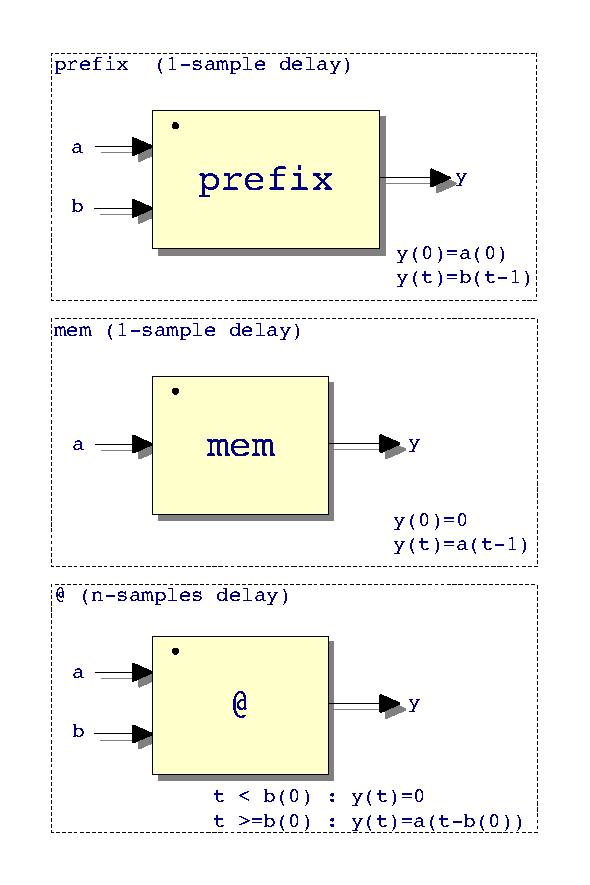
\includegraphics[scale=0.6]{illustrations/faust-diagram4}
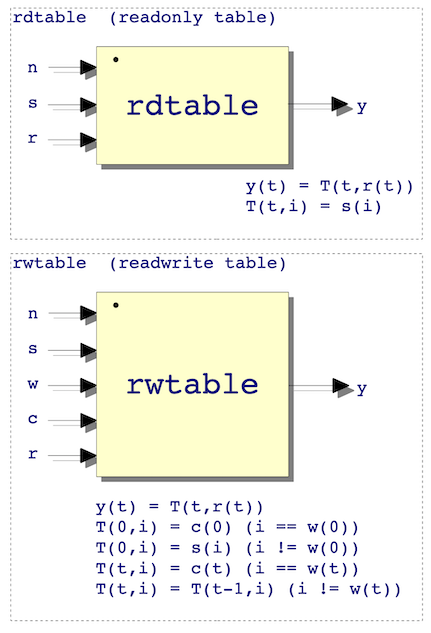
\includegraphics[scale=0.6]{illustrations/faust-diagram5}
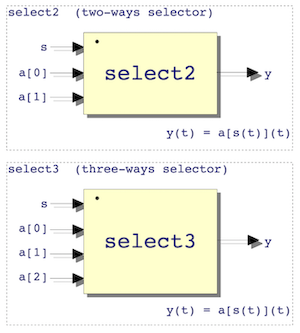
\includegraphics[scale=0.6]{illustrations/faust-diagram6}
\caption{Delays, tables and selectors primitives }
\label{fig-delays}
\end{figure}

The size input of \textit{rdtable} and \textit{rwtable} are \textit{constant numerical expressions}.

%--------------------------------------------------------------------------------------------------------------
\subsection{User Interface Elements}
%--------------------------------------------------------------------------------------------------------------

\faust user interface widgets allow an abstract description of the user interface from within the \faust code. This description is
independent of any GUI toolkits. It is based on \emph{buttons}, \emph{checkboxes}, \emph{sliders}, etc. that are grouped together 
vertically and horizontally using appropriate grouping schemes.

All these GUI elements produce signals. A button for example (see figure \ref{fig-button}) produces a signal which is 1 when the button is pressed and 0 otherwise. These signals can be freely combined with other audio signals. 

\begin{figure}[h]
\centering
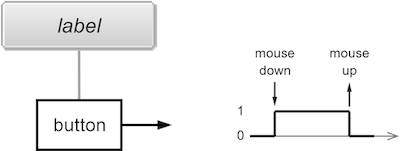
\includegraphics[scale=0.5]{illustrations/button}
\caption{User Interface Button}
\label{fig-button}
\end{figure}

\bigskip

\begin{tabular}{|l|l|}
\hline
\textbf{Syntax} & \textbf{Example} \\
\hline
\texttt{button(\farg{str})} & \texttt{button("play")}\\
\texttt{checkbox(\farg{str})} & \texttt{checkbox("mute")}\\
\texttt{vslider(\farg{str},\farg{cur},\farg{min},\farg{max},\farg{step})} & \texttt{vslider("vol",50,0,100,1)}\\
\texttt{hslider(\farg{str},\farg{cur},\farg{min},\farg{max},\farg{step})} & \texttt{hslider("vol",0.5,0,1,0.01)}\\
\texttt{nentry(\farg{str},\farg{cur},\farg{min},\farg{max},\farg{step})} & \texttt{nentry("freq",440,0,8000,1)}\\
\texttt{vgroup(\farg{str},\farg{block-diagram})} & \texttt{vgroup("reverb", \ldots)}\\
\texttt{hgroup(\farg{str},\farg{block-diagram})} & \texttt{hgroup("mixer", \ldots)}\\
\texttt{tgroup(\farg{str},\farg{block-diagram})} & \texttt{tgroup("parametric", \ldots)}\\
\texttt{vbargraph(\farg{str},\farg{min},\farg{max})} & \texttt{vbargraph("input",0,100)}\\
\texttt{hbargraph(\farg{str},\farg{min},\farg{max})} & \texttt{hbargraph("signal",0,1.0)}\\
\texttt{attach} & \texttt{attach(x, vumeter(x))}\\
\hline
\end{tabular}

All numerical parameters (like {\it cur}, {\it min}, {\it max}, {\it step}) are \textit{constant numerical expressions}.

\bigskip
\subsubsection{Labels}
Every user interface widget has a label (a string) that identifies it and informs the user of its purpose. There are three important mechanisms associated with labels (and coded inside the string): \textit{variable parts}, \textit{pathnames} and \textit{metadata}.

\paragraph{Variable parts.}
Labels can contain variable parts. These variable parts are indicated by the sign '\texttt{\%}' followed by the name of a variable. During compilation each label is processed in order to replace the variable parts by the value of the variable. 
For example \lstinline'par(i,8,hslider("Voice %i", 0.9, 0, 1, 0.01))' creates 8 different sliders in parallel :

\begin{lstlisting}
hslider("Voice 0", 0.9, 0, 1, 0.01),
hslider("Voice 1", 0.9, 0, 1, 0.01),
...
hslider("Voice 7", 0.9, 0, 1, 0.01).
\end{lstlisting}

while \lstinline'par(i,8,hslider("Voice", 0.9, 0, 1, 0.01))' would have created only one slider and duplicated its output 8 times.

The variable part can have an optional format digit. 
For example \lstinline'"Voice %2i"' would indicate to use two digit when inserting the value of i in the string.

An escape mechanism is provided.
If the sign \lstinline'%' is followed by itself, it will be included in the resulting string.
For example \lstinline'"feedback (%%)"' will result in \lstinline'"feedback (%)"'.

The variable name can be enclosed in curly brackets to clearly separate it from the rest of the string, as in \lstinline'par(i,8,hslider("Voice %{i}", 0.9, 0, 1, 0.01))'.



\paragraph{Pathnames.}
Thanks to horizontal, vertical and tabs groups, user interfaces have a hierarchical structure analog to a hierarchical file system. Each widget has an associated \textit{pathname} obtained by concatenating the labels of all its surrounding groups with its own label.

In the following example:
\begin{lstlisting}
hgroup("Foo",
	...
	vgroup("Faa", 
		...
		hslider("volume",...)
		...
	)
	...
)
\end{lstlisting}
the volume slider has pathname \lstinline'/h:Foo/v:Faa/volume'.

In order to give more flexibility to the design of user interfaces, it is possible to explicitly specify the absolute or relative pathname of a widget directly in its label. 

In our previous example the pathname of:
\begin{lstlisting}
	hslider("../volume",...)
\end{lstlisting}
would have been \lstinline'"/h:Foo/volume"', while the pathname of:
\begin{lstlisting}
	hslider("t:Fii/volume",...)
\end{lstlisting}
would have been: 
\lstinline'"/h:Foo/v:Faa/t:Fii/volume"'.

The grammar for labels with pathnames is the following:
% \begin{grammar}
%   <label> ::= 
%   \begin{syntdiag}
% 	<path> <name>
%   \end{syntdiag}
% \end{grammar}
% %
% \begin{grammar}
%  <path> ::= 
%   \begin{syntdiag}
% 	\begin{stack} \\ "/" \end{stack} 
% 	\begin{stack} \\ \begin{rep} <folder> "/" \end{rep} \end{stack} 
%  \end{syntdiag}
% \end{grammar}
% %
% \begin{grammar}
%  <folder> ::= 
%   \begin{syntdiag}
% 	\begin{stack}
% 		".." \\ 
% 		\begin{stack} "h:" \\ "v:" \\ "t:" \end{stack} <name>
% 	\end{stack}
%  \end{syntdiag}
% \end{grammar}

\begin{rail}
 label : path name;
 path : (| '/') (| (folder '/')+);
 folder : (".." | ("h:" | "v:" | "t:" ) name);
\end{rail}

\paragraph{Metadata}
Widget labels can contain metadata enclosed in square brackets. These metadata associate a key with a value and are used to provide additional information to the architecture file.  They are typically used to improve the look and feel of the user interface. 
The \faust code:
\begin{lstlisting}
process = *(hslider("foo [key1: val 1][key2: val 2]", 
					0, 0, 1, 0.1));
\end{lstlisting}

will produce and the corresponding C++ code:

\begin{lstlisting}
class mydsp : public dsp {
	...
	virtual void buildUserInterface(UI* interface) {
	  interface->openVerticalBox("m");
	  interface->declare(&fslider0, "key1", "val 1");
	  interface->declare(&fslider0, "key2", "val 2");
	  interface->addHorizontalSlider("foo", 
	  	&fslider0, 0.0f, 0.0f, 1.0f, 0.1f);
	  interface->closeBox();
	}
...
};
\end{lstlisting}

All the metadata are removed from the label by the compiler and 
transformed in calls to the \lstinline'UI::declare()' method. All these 
\lstinline'UI::declare()' calls will always take place before the \lstinline'UI::AddSomething()' 
call that creates the User Interface element. This allows the 
\lstinline'UI::AddSomething()'  method to make full use of the available metadata.

It is the role of the architecture file to decide what to do with these 
metadata. The \lstinline'jack-qt.cpp' architecture file for example implements the 
following:
\begin{enumerate}
\item \lstinline'"...[style:knob]..."' creates a rotating knob instead of a regular 
slider or nentry.
\item \lstinline'"...[style:led]..."' in a bargraph's label creates a small LED instead 
of a full bargraph
\item \lstinline'"...[unit:dB]..."' in a bargraph's label creates a more realistic 
bargraph with colors ranging from green to red depending of the level of 
the value
\item \lstinline'"...[unit:xx]..."' in a widget postfixes the value displayed with xx
\item \lstinline'"...[tooltip:bla bla]..."' add a tooltip to the widget
\item \lstinline'"...[osc:/address min max]..."' Open Sound Control message alias
\end{enumerate}

Moreover starting a label with a number option like in \lstinline'"[1]..."' provides
a convenient means to control the alphabetical order of the widgets.

\subsubsection{Attach}
The \lstinline'attach' primitive takes two input signals and produce one output signal which is a copy of the first input. The role of \lstinline'attach' is to force its second input signal to be compiled with the first one. From a mathematical point of view \lstinline'attach(x,y)' is equivalent to \lstinline'1*x+0*y', which is in turn equivalent to \lstinline'x', but it tells the compiler not to optimize-out \lstinline'y'.

To illustrate this role let say that we want to develop a mixer application with a vumeter for each input signals. Such vumeters can be easily coded in \faust using an envelop detector connected to a bargraph. The problem is that these envelop signals have no role in the output signals. Using \lstinline'attach(x,vumeter(x))' one can tell the compiler that when \lstinline'x' is compiled \lstinline'vumeter(x)' should also be compiled. 


